% Seta a imagem do capítulo
\chapterimage{chapter_head_2.pdf}
% O título e rótulo do cabiluto
\chapter{Relações}\label{cap:Relacoes}

%\epigraph{``-Se não faz sentido''. Disse o rei.\\``-Isso nos poupa de uma montanha de trabalho não é? Pois assim não precisamos ficar tentando encontrar sentido ai.''}{Lewis Carroll, Alice no País das Maravilhas.}

%\epigraph{``Nunca imaginei que você mesma não é outra coisa senão o que poderia parecer a outros do que o que você fosse ou poderia ter sido não fosse senão o que você tivesse sido teria parecido a eles ser de outra maneira.''}{Lewis Carroll, Alice no País das Maravilhas.}

%\epigraph{``A única coisa perfeita é o conjunto vazio.''}{Elon Lages Lima}

\epigraph{``Mathematics is a language''}{Josiah Willard Gibbs}

\section{Noções Básicas de Relações}\label{sec:RelacaoParOdenado}

A ideia de relação é um conceito frequentemente utilizado, seja no cotidiano das pessoas, seja na matemática \cite{barreto1998}. Uma subárea da matemática de extrema importância para a Ciência da Computação, especificamente na área de banco de dados, é a álgebra relacional, que de forma resumida é o estudo das relações entre objetos de um mesmo espaço (conjunto). 

Como comentado em \cite{sussana2010-MD}, no cotidiano do mundo ``real'' existem diversos tipos de relacionamentos entre as entidades, por exemplo, imagine que duas pessoas, um homem jovem e um(a) garotinho(a) compartilham um ancestral comum, tal como um avô, assim pode-se dizer que os dois apresentam uma relação de parentesco, ou ainda que existe uma relação familiar entre os dois.  

No que diz respeito ao universo matemático a noção de relação entre os objetos é algo onipresente. Um exemplo clássico de relacionamento que pode-se estabelecer entre dois números $x$ e $y$, é a ideia de dobro, isto é, $x$ e $y$ apresentam um relacionamento de dobro entre si no caso de $y = 2x$ ou $x = 2y$.

Note que de forma subliminar os exemplos anteriores caracterizam as relações de parentesco e dobro através da associação de elementos que juntos apresentavam uma certa propriedade, e nesse sentido uma relação nada mais é do que um conjunto definido sobre um certa propriedade entre elementos de um espaço. A formalização das relações como sendo um conjunto será construída nas próximas seções.

\section{Pares Ordenados e Produto Cartesiano}\label{sec:ParesOrdenadoEProduto}

Da mesma forma que \cite{abe1991-TC}, neste manuscrito será considera a definição apresentada a seguir de par ordenado, sendo que tal definição foi apresentada pela primeira vez pelo grande matemático e lógico polonês Kazimierz Kuratowski (1896--1980).

\begin{definition}[Par ordenado]\label{def:ParOrdenado}
	Sejam $x$ e $y$ elementos em um universo do discurso. O par ordenado entre $x$ e $y$, denotado por $(x, y)$, corresponde a seguinte igualdade.
	\begin{eqnarray*}
		(x, y) = \{x, \{x, y\}\}
	\end{eqnarray*}
\end{definition}

Dado qualquer par ordenado $(x,y)$ o elemento $x$ é chamado de primeira componente do par ordenado, e o $y$ é chamado de segunda componente do par ordenado. Além disso, como explicado em \cite{lipschutz2013-MD, lipschutz1978-TC} a propriedade fundamental dos pares ordenados diz que, dois pares ordenados $(x_1, y_1)$ e $(x_2, y_2)$ serão iguais\footnote{Este resultado  segue da definição de igualdade de conjuntos (ver \ref{def:IgualdadeConjuntos}), provar tal igualdade é um exercício interessante ao leitor.},  isto é, $(x_1, y_1) = (x_2, y_2)$ se, e somente se, $x_1 = x_2$ e $y_1 = y_2$.

\begin{rema}
	O leitor deve ficar atento na distinção que existe entre o par ordenado $(x,y)$ e o conjunto $\{x, y\}$. Apesar de ambos terem os mesmo elementos básico, são objetos matemáticos distintos.
\end{rema}

De posse do conceito de par ordenado é possível definir uma nova operação sobre conjuntos, tal operação recebe o nome de produto Cartesiano\footnote{O nome produto Cartesiano provém do matemática francês René Descartes (1596--1650), que foi o primeiro a estudar tal operação conjuntista \cite{lipschutz1978-TC}.} e será de vital importância para em seguida apresentar as ideias ligadas ao conceito de relações.

\begin{definition}[Produto Cartesiano]\label{def:ProdutoCartesiano}
	Sejam $A$ e $B$ dois conjuntos quaisquer. O produto Cartesiano de $A$ e $B$, denotado por $A \times B$, corresponde ao conjunto de todos os pares ordenado onde a primeira componente é um elemento de $A$ e a segunda componente é um elemento de $B$, em notação formal tem-se que:
	\begin{eqnarray*}
		A \times B = \{(x, y) \mid x \in A, y \in B\}
	\end{eqnarray*}
\end{definition}

\begin{exem}\label{exe:ProdutoCartesiano1}
	Dado os seguintes dois conjuntos $\{a, b, c\}$ e $\{-1, 1\}$ tem-se os seguintes produtos Cartesianos:
	\begin{itemize}
		\item[(a)] $\{a, b, c\} \times \{-1, 1\}  = \{(a, 1), (a, -1), (b, -1), (b, 1), (c, -1), (c, 1)\}$.
		\item[(b)] $\{-1, 1\} \times \{a, b, c\}  = \{(1, a), (1, b), (1, c), (-1, a), (-1, c), (-1, b)\}$.
		\item[(c)] $\{a, b, c\} \times \{a, b, c\}   = \{(a, a), (a, b), (a, c), (b, a), (b, b), (b, c), (c, a), (c, b), (c, c)\}$.
		\item[(d)] $\{-1, 1\} \times \{-1, 1\} = \{(1, 1), (1, -1), (-1, 1), (-1, -1)\}$.
	\end{itemize}
\end{exem}

Um caso particular do produto Cartesiano e o chamado Cartesiano quadrado apresentado a seguir.

\begin{definition}[Cartesiano quadrado]\label{def:CartesianoQuadrado}
	Seja $A$ um conjunto qualquer. O produto Cartesiano quadrado de $A$, denotado por $A \times A$ ou ainda por $A^2$, corresponde ao produto Cartesiano de A consigo mesmo, em notação formal tem-se que:
	\begin{eqnarray*}
		A^2 = \{(x, y) \mid x, y \in A\}
	\end{eqnarray*}
\end{definition}

\begin{rema}
	Neste manuscrito o produto Cartesiano quadrado de um conjunto $A$ será denotado, sempre que possível, pela notação $A^2$.
\end{rema}

\begin{exem}\label{exe:ProdutoCartesiano2}
	Os itens $(c)$ e $(d)$ do Exemplo \ref{exe:ProdutoCartesiano1} são resultados do produto Cartesiano quadrado aplicada respectivamente aos conjuntos $\{a, b, c\}$ e $\{-1, 1\}$.
\end{exem}

\begin{theorem}[Produto Cartesiano - absorção]\label{teo:AbsorcaoCatersiano}
	Dado dois conjuntos $A$ e $B$ tem-se que, $A \times B = \emptyset$ se, e somente se, $A = \emptyset$ ou $B = \emptyset$.
\end{theorem}

\begin{proof}
	$(\Rightarrow)$ Por contrapositiva assuma que $A \neq \emptyset$ e $B \neq \emptyset$, assim tem-se que existem $x \in A$ e $y \in B$, consequentemente, pela definição de produto cartesiano existe $(x,y) \in A \times B$, assim tem-se que, $A \times B \neq \emptyset$, e portanto, a afirmação: Se $A \times B = \emptyset$, então $A = \emptyset$ ou $B = \emptyset$ é verdadeira.
	
	$(\Leftarrow)$ Suponha que $A = \emptyset$ ou $B = \emptyset$, assim por vacuidade é claro que $A \times B = \emptyset$.
\end{proof}

\begin{theorem}[Produto Cartesiano - igualdade]\label{teo:IgualdadeCartesiano}
	Dado dois conjuntos $A$ e $B$ tem-se que, $A \times B = B \times A$ se, e somente se, $A = \emptyset$ ou $B = \emptyset$ ou $A = B$.
\end{theorem}

\begin{proof}
	A prova deste enunciado irá ficar como exercício ao leitor.
\end{proof}

O produto Cartesiano enquanto operação tem a propriedade de preservar a relação de inclusão à direta e à esquerda como pode ser visto a seguir.

\begin{theorem}[Produto Cartesiano - monotonicidade à direita]\label{teo:CartesianoMonoDireita}
	Dado três conjuntos $A, B$ e $C$ tem-se que, $A \subset B$ se, e somente se, $A \times C \subset B \times C$.
\end{theorem}

\begin{proof}
	$(\Rightarrow)$ Suponha que $A \subset B$, logo por definição tem-se que todo $x \in A$ é tal que $x \in B$, e assim é óbvio que para todo $(x,y) \in A \times C$ tem-se que $(x, y) \in B \times C$, e portanto, pela definição de subconjunto tem-se que $A \times C \subseteq B \times C$, mas por hipótese tem-se que existe $x' \in B$ tal que $x' \notin A$, logo existe $(x', y) \in B \times C$ tal que $(x', y) \notin A \times C$, consequentemente, $A \times C \subset B \times C$.
	
	$(\Leftarrow)$ Assuma que $A \times C \subset B \times C$, logo tem-se que para todo $(x, y) \in A \times C$ tem-se que $(x, y) \in B \times C$, mas note que por definição $(x, y) \in A \times C$ se, e somente se, $x \in A$ e de forma similar tem-se que $(x, y) \in B \times C$ se, e somente se, $x \in B$, dessa forma tem-se que $A \subset B$, além disso, por hipótese existe um $(x', y) \in B \times C$ tal que $(x', y) \notin A \times C$, portanto, é claro que existe $x' \in B$ tal que $x' \notin A$, consequentemente, $A \subset B$.
\end{proof}

\begin{theorem}[Produto Cartesiano - monotonicidade à esquerda]
	Dado três conjuntos $A, B$ e $C$ tem-se que, $A \subset B$ se, e somente se, $C \times A \subset C \times B$.
\end{theorem}

\begin{proof}
	Similar a demonstração do Teorema \ref{teo:CartesianoMonoDireita}.
\end{proof}

%O próximo resultado mostra que a operação de produto Cartesiano se distribui sobre as operações de união, interseção e diferença.

\begin{theorem}[Leis de Distributividade do Cartesiano]\label{teo:DistributividadeCartesiano}
	Dado três conjuntos $A, B$ e $C$ tem-se que:
	\begin{itemize}
		\item[(i)] $A \times (B \cap C) = (A \times B) \cap (A \times C)$.
		\item[(ii)] $(A \cap B) \times C = (A \times C) \cap (B \times C)$.
		\item[(iii)] $A \times (B \cup C) = (A \times B) \cup (A \times C)$.
		\item[(iv)] $(A \cup B) \times C = (A \times C) \cup (B \times C)$.
		\item[(v)] $A \times (B - C) = (A \times B) - (A \times C)$.
		\item[(vi)] $(A - B) \times C = (A \times C) - (B \times C)$.
		\item[(vii)] $A \times (B \ominus C) = (A \times B) \ominus (A \times C)$.
		\item[(vii)] $(A \ominus B) \times C = (A \times C) \ominus (B \times C)$.
	\end{itemize}
\end{theorem}

\

\begin{proof}
	Sejam $A, B$ e $C$ conjuntos tem-se que:
	\begin{itemize}
		\item[(i)] 
		\begin{eqnarray*}
			A \times (B \cap C) & = & \{(x, y) \mid x \in A, y \in (B \cap C)\}\\
			& = & \{(x, y) \mid x \in (A \cap A), y \in (B \cap C)\}\\
			& = & \{(x, y) \mid x \in A, x \in A, y \in B, y \in C\}\\
			& = & \{(x, y) \mid x \in A, y \in B, x \in A, y \in C\}\\
			& = & \{(x, y) \mid x \in A, y \in B\} \cap \{(x, y) \mid x \in A, y \in C\}\\
			& = & (A \times B) \cap (A \times C)
		\end{eqnarray*}
		\item[(ii)] Similar ao item anterior.
		\item[(iii)]
		\begin{eqnarray*}
			A \times (B \cup C) & = & \{(x, y) \mid x \in A, y \in (B \cup C)\}\\
			& = & \{(x, y) \mid x \in (A \cup A), y \in (B \cup C)\}\\
			& = & \{(x, y) \mid x \in A \text{ ou } x \in A, y \in B \text{ ou } y \in C\}\\
			& = & \{(x, y) \mid x \in A, y \in B \text{ ou } x \in A, y \in C\}\\
			& = & \{(x, y) \mid x \in A, y \in B\} \cup \{(x, y) \mid x \in A, y \in C\}\\
			& = & (A \times B) \cup (A \times C)
		\end{eqnarray*}
		\item[(iv)] Similar ao item anterior.
		\item[(v)]
		\begin{eqnarray*}
			A \times (B - C) & = & \{(x, y) \mid x \in A, y \in (B-C)\}\\
			& = & \{(x, y) \mid x \in A \cap A, y \in (B-C)\}\\
			& = & \{(x, y) \mid x \in A, x \in A, y \in B, y \notin C\}\\
			& = & \{(x, y) \mid (x, y) \in A \times B, (x, y) \notin (A \times  C)\}\\
			& = & (A \times B) - (A \times C)
		\end{eqnarray*}
		\item[(vi)] Similar ao item anterior.
		\item[(vii)]
		\begin{eqnarray*}
			A \times (B \ominus C) & \stackrel{Cor. \ \ref{col:DiferencaSimetrica}}{=} & A \times ((B \cup C) - (B \cap C))\\
			& \stackrel{Teo. \ \ref{teo:DistributividadeCartesiano}(\text{v})}{=} & (A \times (B \cup C)) - (A \times (B \cap C))\\
			& \stackrel{Teo. \ \ref{teo:DistributividadeCartesiano}(\text{iii})}{=} & ((A \times B) \cup (A \times C)) - (A \times (B \cap C))\\
			& \stackrel{Teo. \ \ref{teo:DistributividadeCartesiano}(\text{i})}{=} & ((A \times B) \cup (A \times C)) - ((A \times B) \cap (A \times C))\\
			& \stackrel{Cor. \ \ref{col:DiferencaSimetrica}}{=} & (A \times B) \ominus (A \times C)
		\end{eqnarray*}
		\item[(viii)] Similar ao item anterior.
	\end{itemize}
\end{proof}


O conceito do produto Cartesiano pode, como explicado em \cite{lipschutz1978-TC, lipschutz2013-MD}, ser estendido a poder operar com mais de dois conjuntos, sendo essa extensão realizada de forma natural apenas aumentando um número de componentes nos elementos do conjunto resultante ao conjunto do produto, ou seja, os elementos deixam de ser simples pares ordenados para serem tuplas ordenadas. A seguir este conceito é formalizado.

\begin{definition}[Produto Cartesiano $n$-ário]
	Dado $n \geq 2$ e sejam $A_1, A_2, \cdots, A_n$ conjuntos quaisquer, o produto Cartesiano $n$-ário, denotado por $A_1 \times \cdots \times A_n$, corresponde ao conjunto formado por todas as tuplas da forma $(a_1, \cdots, a_n)$ tal que para todo $1 \leq i \leq n$ tem-se que $a_i \in A_i$.
\end{definition}

\

\begin{rema}
	Outra forma comum de denotar o produto Cartesiano $n$-ário muito encontrada na literatura é usando o símbolo do produtório, ou seja, $\displaystyle\prod_{i = 1}^{n} A_i$ 
\end{rema}

Em um produto Cartesiano $n$-ário da forma $A_1 \times \cdots \times A_n$ cada $A_i$ com $1 \leq i \leq n$ é chamado de $i$-ésimo fator do produto. No caso particular em que $A_1 = A_2 = \cdots = A_n$ o produto Cartesiano $n$-ário é escrito simplesmente como $A^n$.

\begin{exem}\label{exe:CartesianoNario1}
	Dado os conjuntos $\{-1, 1\}, \{a, b\}$ e $\{0, 1\}$ tem-se os seguintes produtos Cartesianos $n$-ários:
	\begin{eqnarray*}
		\{-1, 1\} \times \{a, b\} \times \{0, 1\} & = & \{(-1, a, 0), (-1, a, 1), (-1, b, 0), (-1, b, 1), \\
		& & \ \ (1, a, 0), (1, a, 1), (1, b, 0), (1, b, 1)\}
	\end{eqnarray*}
	\begin{eqnarray*}
		\{-1, 1\} \times \{-1, 1\} \times \{a, b\} \times \{a, b\} & = & \{ (-1, 1, a, a), (-1, 1, a, b), \\
		& & \ \ (-1, 1, b, a),  (-1, 1, b, b), \\
		& & \ \ (-1, -1, a, a), (-1, -1, a, b),\\
		& & \ \ (-1, -1, b, a), (-1, -1, b, b),\\
		& & \ \ (1, -1, a, a),  (1, -1, a, b),\\
		& & \ \ (1, -1, b, a),  (1, -1, b, b),\\
		& & \ \ (1, 1, a, a),   (1, 1, a, b),\\
		& & \ \ (1, 1, b, a),   (1, 1, b, b) \}
	\end{eqnarray*}
\end{exem}

\begin{exem}\label{exe:CartesianoNario2}
	Dado o conjunto $\{0,1\}$ tem-se que 
	\begin{eqnarray*}
		\{0, 1\}^5 & = & \{ (0, 0, 0, 0, 0), (0, 0, 0, 0, 1), (0, 0, 0, 1, 0), (0, 0, 0, 1, 1), (0, 0, 1, 0, 0), (0, 0, 1, 0, 1),\\
		& & \ \ (0, 0, 1, 1, 0), (0, 0, 1, 1, 1), (0, 1, 0, 0, 0), (0, 1, 0, 0, 1), (0, 1, 0, 1, 0), (0, 1, 0, 1, 1),\\
		& & \ \ (0, 1, 1, 0, 0), (0, 1, 1, 0, 1), (0, 1, 1, 1, 0), (0, 1, 1, 1, 1), (1, 0, 0, 0, 0), (1, 0, 0, 0, 1),\\
		& & \ \ (1, 0, 0, 1, 0), (1, 0, 0, 1, 1), (1, 0, 1, 0, 0), (1, 0, 1, 0, 1), (1, 0, 1, 1, 0), (1, 0, 1, 1, 1),\\
		& & \ \ (1, 1, 0, 0, 0), (1, 1, 0, 0, 1), (1, 1, 0, 1, 0), (1, 1, 0, 1, 1), (1, 1, 1, 0, 0), (1, 1, 1, 0, 1),\\
		& & \ \ (1, 1, 1, 1, 0), (1, 1, 1, 1, 1)\}\\
	\end{eqnarray*}
\end{exem}

Quando os conjuntos $A_1, A_2, \cdots, A_n$ são todos conjuntos finitos, uma estratégia muito utilizada para se obter e também representar o mecanismo de construção das tuplas $(a_1, a_2, \cdots, a_n)$ pertencentes ao produto Cartesiano $n$-ário $A_1 \times A_2 \times \cdots \times A_n$ é usando a noção de diagrama de árvore \cite{lipschutz1978-TC, lipschutz2013-MD}.

\begin{rema}
	De forma contrária ao que acontecer nos diagramas de árvores nas área de estrutura de dados \cite{jaime1994}, linguagens formais \cite{benjaLivro2010, hopcroft2008, linz2006}  e compiladores \cite{aho2007, cooper2017}, os diagramas de árvore na teoria dos conjuntos são construídos de forma horizontal no sentido da esquerda para à direita.
\end{rema}

Em um diagrama de árvore o número de níveis na árvore é igual ao número de conjuntos envolvidos no Cartesiano mais 2, ou seja, para cada produto Cartesiano $n$-ário, o número de níveis na árvore que gera/representa tal cartesiano é igual a $n+2$. O diagrama é construindo por níveis da seguinte forma: Seguido a sequência dos conjuntos no Cartesiano $A_1 \times \cdots \times A_n$, para todo $1 \leq i \leq n$ cada nível $i$ do diagrama de árvore vai ser preenchido pelos elementos do conjunto $A_i$, com o conjunto $A_i$ sendo repetido exatamente $2^{i-1}$ vezes a cada nível $i$, no nível inicial da árvore (nível 0) é colocado o símbolo de inicio da árvore, neste manuscrito será usado o $\ast$ como símbolo inicial, e no último nível da árvore (ou nível EPC) estão os elementos do produto Cartesiano em si. 
 
\begin{exem}\label{exe:ArvoreDoCartesino}
	Dado os conjuntos $\{-1, 1\}, \{a, b\}$ e $\{-1, 1\}$ tem-se que o produto Cartesiano $\{-1, 1\} \times \{a, b\} \times \{-1, 1\}$ pode ser representado pelo diagrama a seguir.
	\begin{figure}[h]
		\begin{tikzpicture}[grow'=right,level distance=1.25in,sibling distance=.25in]
			\tikzset{edge from parent/.style= {thick, draw, edge from parent fork right}, every tree node/.style={align=center}}
			\Tree 
			[. $\ast$
				[.{$-1$}
					[.{$a$}
						[.{$-1$}
							[.{$(-1, a, -1)$} ]  
						]
						[.{$1$} 
							[.{$(-1, a, 1)$} ] 
						] 
					]
					[.{$b$} 
						[.{$-1$} 
							[.{$(-1, b, -1)$} ]   
						]
						[.{$1$} 
							[.{$(-1, a, 1)$} ] 	
						]
					]
				]
				[.{$1$}
					[.{$a$}
						[.{$-1$} 
							[.{$(1, a, -1)$} ]  
						]
						[.{$1$} 
							[.{$(1, a, 1)$} ]
						] 
					]
					[.{$b$} 
						[.{$-1$} 
							[.{$(1, b, -1)$} ]  
						]
						[.{$1$} 
							[.{$(1, b, 1)$} ]
						]
					]
				]
			]
			\begin{scope}[yshift=-6cm]
				\Tree 
				[.{nível 0} [.{nível 1} [.{nível 2} [.{nível 3} [.{EPC} ] ] ]  ] ]
			\end{scope}
		\end{tikzpicture}
		\caption{Diagrama de árvore para o Cartesiano $\{a, b\} \times \{1, -1\} \times \{1, -1\}$.}
		\label{fig:Cartesiano}
	\end{figure}
	%\tikzset{edge from parent/.style= {thick, draw, edge from parent fork right},every tree node/.style={draw,minimum width=1in,text width=1in,align=center}}
\end{exem}

Apesar de ser uma ótima forma prática de representar e visualizar o produto Cartesiano, os diagramas de árvores tendem a não ser adotados com frequência pois seu crescimento se dá em proporções fatoriais, o que torna sua construção facilmente complexa.

\begin{rema}
	Para finalizar o tópico ligado ao produto Cartesiano o leitor deve ficar atento a alguns fatos de cunho sintático\footnote{Ótimas discussões sobre esses aspectos sintáticos do produto Cartesiano ocorreram de forma breve nas páginas \url{encurtador.com.br/cdjBY} e \url{encurtador.com.br/pJLRZ}.} a respeito do produto Cartesiano, por exemplo, note que $A \times B \times C \neq A \times (B \times C) \neq (A \times B) \times C$. No primeiro produto os elementos gerados são da forma $(x, y, z)$, já no segundo os elementos terão a forma $(x, (y, z))$, e por fim, no terceiro produto os elementos tem a seguinte forma $((x,y), z)$ sendo $x \in A, y \in B$ e $z \in C$. Além disso, tem-se que o produto Cartesiano $A^n \times B = (\underbrace{A \times \cdots \times A}_{n-\text{vezes}}) \times B$. 
\end{rema}

\section{Relações}\label{sec:Relacoes}

Da mesma forma que foi apresentado em \cite{abe1991-TC}, este manuscrito irá iniciar tratando de relações binária e depois será feita uma apresentação para as relações $n$-árias. Assim esta seção inicia apresentando formalmente o conceito de relação binária como se segue.

\begin{definition}[Relação binária]\label{def:RelacaoBinaria}
	Seja $A$ e $B$ dois conjuntos, uma relação $R$ de $A$ em $B$ é qualquer subconjunto de $A \times B$, isto é, $R \subseteq (A \times B)$.
\end{definition}

Sendo $R$ uma relação binária de $A$ em $B$ é comum adotar a notação $x\mathrel{R}y$ para especificar a relação de pertinência $(x,y) \in R$, e é usado a notação $x\centernot{R}y$ para especificar que $(x,y) \notin R$, sendo que $x\mathrel{R}y$ pode ser lido como, ``$x$ está $R$-relacionado (está relacionado por $R$) com $y$'', e sendo  $x\centernot{R}y$ lido como, ``$x$ não está $R$-relacionado (não está relacionado por $R$) com $y$''.

\begin{rema}
	Em algumas obras como \cite{carmo2013}, é possível ver a notação $x \underrightarrow{R} y$ para dizer que $(x, y) \in R$.
\end{rema}

\begin{rema}
	Quando $R \subseteq A \times A$ é dito simplesmente que $R$ é uma relação sobre $A$, em vez de dizer que $R$ é uma relação de $A$ em $A$.
\end{rema}

Este manuscrito irá continuar definido dois objetos fundamentais no estudo das relações binárias, que são respectivamente o domínio e a imagem.

\begin{definition}[Domínio e Imagem]\label{def:DominioImagemRelacoes}
	Seja $R$ uma relação de $A$ em $B$, o domínio de $R$, denotado por $Dom(R)$, corresponde ao conjunto de todos os elementos de $A$ que são a primeira coordenada de $x\mathrel{R}y$, ou seja, 
	$$Dom(R) = \{x \in A \mid x\mathrel{R}y\}$$
 	e a imagem de $R$, denotada por $Ima(R)$, corresponde ao conjunto de todos os elementos de $B$ que são a segunda coordenada de $x\mathrel{R}y$, ou seja, 
	$$Ima(R) = \{y \in B \mid x\mathrel{R}y\}$$
\end{definition}

\begin{exem}\label{exe:RelacaoBinaria1}
	Seja $R = \{(a, 1), (b, -1), (c, 1), (b, 1), (c, -1)\}$ uma relação tem-se que $Dom(R) = \{a, b, c\}$ e $Ima(R) = \{1, -1\}$.
\end{exem}

\begin{exem}
	Dado a relação $Q = \{(x, y) \in \mathbb{N}^2 \mid x^2 = y\}$ tem-se que $Dom(Q) = \{x \in \mathbb{N} \mid (\exists y \in \mathbb{N})[\sqrt{y} = x]\}$ e $Ima(Q) = \{y \in \mathbb{N} \mid (\exists x \in \mathbb{N})[x^2 = y]\}$
\end{exem}

\begin{exem}
	Uma relação binária $R$ famosa é aquela usada para representar o conjunto das frações positivas, tal relação é definida como $F = \{(x, y)\mid x \in \mathbb{N}, y \in (\mathbb{N}-\{0\})\}$, note que a fração $\displaystyle\frac{1}{12}$ por exemplo corresponde ao elemento $1\mathrel{F}12$.
\end{exem}

Dada qualquer relação $R$ sempre é possível obter uma nova relação a partir de $R$, essa nova relação recebe o nome de relação inversa ou oposta.

\begin{definition}[Relação inversa]\label{def:RelacaoInversa}
	Seja $R$ uma relação. A relação inversa (ou oposta) de $R$, denotada por $R^{-1}$, corresponde ao seguinte conjunto:
	$$R^{-1} = \{(y,x) \mid x\mathrel{R}y\}$$
\end{definition}

\begin{exem}
	Considere a relação $R$ do Exemplo \ref{exe:RelacaoBinaria1}, tem-se que a relação inversa de $R$ corresponde ao conjunto $R^{-1} = \{(1, a), (-1, b), (1, c), (-1, c), (1, b)\}$.
\end{exem}

Uma vez que relações são conjuntos pode-se falar sobre as operações sobre relações, aqui não serão tratadas as operações triviais de união, interseção, complemento e diferença. Para essas operações é recomendável que o leitor retorne para revisar o texto apresentado na Seção \ref{sec:OperacoesConjuntos} que trata exatamente de tais operações. 

Uma operação natural que surge para as relações é a noção de composição entre duas relações $R_1$ e $R_2$, a ideia da composição é gerar uma terceira relação a partir das relações iniciais. A seguir este manuscrito apresenta formalmente o conceito de composição.

\begin{definition}[Composição de relações]\label{def:ComposicaoRelacoes}
	Seja $R_1$ uma relação de $A$ em $B$ e seja $R_2$ uma relação de $B$ em $C$, a composição de $R_1$ e $R_2$, denotada por $R_1 \bullet R_2$, corresponde ao seguinte conjunto:
	$$R_1 \bullet R_2 = \{(x, z) \mid (\exists y \in B)[x\mathrel{R_1}y \text{ e } y\mathrel{R_2}z] \}$$ 
\end{definition}

\begin{prop}
	Seja $R_1$ uma relação de $A$ em $B$ e seja $R_2$ uma relação de $B$ em $C$, então tem-se que:
	\begin{itemize}
		\item[(i)] $Dom(R_1 \bullet R_2) \subseteq Dom(R_1)$.
		\item[(ii)] $Ima(R_1 \bullet R_2) \subseteq Ima(R_2)$.
	\end{itemize}
\end{prop}

\begin{proof}
	Trivial pela própria Definição \ref{def:ComposicaoRelacoes}.
\end{proof}

\begin{exem}
	Sejam $R = A \times B$ e $Q = B \times C$ tem-se que $R \bullet Q = A \times C$.
\end{exem}

\begin{exem}
	Sejam $R_1 = \{(a, b), (i, b), (o, c), (o, e)\}$ e $R_2 = \{(b, 1), (b, -1), (c, 3), (d, 4)\}$ tem-se então que a composição de $R_1$ e $R_2$ é exatamente igual a relação $R = \{(a, 1), (a, -1),$ $(i, 1), (i, -1), (o, 3)\}$.
\end{exem}

\begin{theorem}[Monotonicidade da Composição de Relações]\label{teo:MonotonicidadeComposicaoRelacoes}
	Seja $R_1$ e $R_2$ relações de $A$ em $B$. Se $R_1 \subseteq R_2$, então para toda relação $R_3$ de $B$ em $C$ tem-se que $(R_1 \bullet R_3) \subseteq (R_2 \bullet R_3)$
\end{theorem}

\begin{proof}
	Suponha que $R_1$ e $R_2$ são ambas relações de $A$ em $B$ e que $R_1 \subseteq R_2$, agora note que para qualquer relação $R_3$ de $B$ em $C$ tem-se por definição que $(x, z) \in (R_1 \bullet R_3)$ se, e somente se, $(\exists y \in B)[x\mathrel{R_1}y \text{ e } y\mathrel{R_3}z]$, mas uma vez que, $R_1 \subseteq R_2$ é claro que $ (\exists y \in B)[x \mathrel{R_2}y \text{ e } y\mathrel{R_3}z]$, e assim $(x, z) \in (R_2 \bullet R_3)$, portanto, $(R_1 \bullet R_3) \subseteq (R_2 \bullet R_3)$, concluindo assim a prova.
\end{proof}

\begin{corollary}\label{col:MonotonicidadeComposicaoRelacoes}
	Se $R_1, R_2, S_1, S_2$ são relações tais que $R_1 \subseteq R_2$ e $S_1 \subseteq S_2$ com $Ima(R_1) = Dom(S_1)$ e $Ima(R_2) = Dom(S_2)$, então $(R_1 \bullet S_1) \subseteq (R_2 \bullet S_2)$.
\end{corollary}

\begin{proof}
	Suponha que $R_1, R_2, S_1, S_2$ são relações tais que $R_1 \subseteq R_2$ e $S_1 \subseteq S_2$ com $Ima(R_1) = Dom(S_1)$ e $Ima(R_2) = Dom(S_2)$, assim pelo Teorema \ref{teo:MonotonicidadeComposicaoRelacoes} tem-se que $(R_1 \bullet S_1) \subseteq (R_2 \bullet S_1)$. Agora note que por definição $(x, z) \in (R_2 \bullet S_1)$ se, e somente se, $(\exists y \in Dom(S_1))[x\mathrel{R_2}y \text{ e } y\mathrel{S_1}z]$, mas uma vez que $S_1 \subseteq S_2$ tem-se que $Dom(S_1) \subseteq Dom(S_2)$ e $Ima(S_1) \subseteq Ima(S_2)$ e assim é claro que $(\exists y \in Dom(S_2))[x\mathrel{R_2}y \text{ e } y\mathrel{S_2}z]$, logo $(x, z) \in (R_2 \bullet S_2)$, consequentemente pela definição de subconjunto tem-se que $(R_2 \bullet S_1) \subseteq (R_2 \bullet S_2)$. E portanto, $(R_1 \bullet S_1) \subseteq (R_2 \bullet S_2)$.
\end{proof}


\section{Tipos e Propriedades das Relações Binárias}

Deste ponto em diante todas as relações consideradas até o final deste capítulo serão relações binárias sobre um conjunto não vazio $A$ genérico, ou seja, tem-se que se $R$ for uma relação, então $R \subseteq A \times A$. Dito isto, pode-se apresentar alguns ``tipos'' em que as relações binárias podem ser classificadas.

\begin{definition}[Tipo Identidade]\label{def:RelacaoIdentica}
	Uma relação $R$ é dita ser relação de identidade (ou relação idêntica \cite{abe1991-TC}) sempre que $R$ é igual ao conjunto $\{(x, x) \mid x \in A\}$.
\end{definition}

\begin{exem}
	Seja $A = \{1, 2, 3, 4\}$ a relação $M = \{(3, 3), (1, 1), (2,2)\}$ é uma relação de identidade, já a relação $Q = \{(1, 1), (2,2), (3,4)\}$ não é uma relações de identidade.
\end{exem}

\begin{rema}
	Quando para todos os $x \in A$ uma relação de identidade possuir exatamente todos os pares da forma $(x, x)$, essa relação é chamada de identidade do conjunto $A$ (ou simplesmente identidade de $A$), e nesse caso tal relação é denotado por $Id_A$.
\end{rema}

\begin{theorem}[Neutralidade da relação de identidade]\label{teo:NeutralidadeRelacaoIdentidade}
	Se $R$ é uma relação sobre $A$, então as seguintes igualdade são verdadeiras:
	\begin{itemize}
		\item[(i)] $R \bullet Id_A = R$.
		\item[(ii)] $Id_A \bullet R = R$.
	\end{itemize}
\end{theorem}

\begin{proof}
	(i) Suponha que $R$ é uma relação sobre $A$, assim tem-se que:
	\begin{eqnarray*}
		(x, y) \in R \bullet Id_A  & \Longleftrightarrow & (\exists y \in A)[x \mathrel{R} y \text{ e } y \mathrel{Id_A} y]\\
		& \Longleftrightarrow & (\exists x \in A)[x \mathrel{R} y]\\
		& \Longleftrightarrow & (x, y) \in R 
	\end{eqnarray*}
	Portanto,  $R \bullet Id_A = R$. (ii) Similar a demonstração do item anterior.
\end{proof}

\begin{prop}\label{prop:ComplementarDaRelacaoIdentica}
	Se $A$ é um conjunto não vazio, então $I_A^{-1} = I_A$.
\end{prop}

\begin{proof}
	Trivial pelas Definições \ref{def:RelacaoInversa} e \ref{def:RelacaoIdentica}.
\end{proof}

\begin{rema}\label{rema:UnicidadeDaRelacaoIdentica}
	É fácil notar que para qualquer que seja o conjunto não vazio $A$ tem-se que a relação identidade $I_A$ é única.
\end{rema}

\begin{definition}[Tipo Reflexivo]\label{def:RelacaoReflexiva}
	Uma relação $R$ é dita ser reflexiva quando para todo $x \in A$ tem-se que $x \mathrel{R} x$.
\end{definition}

Um leitor atento pode perceber que a relação identidade de um conjunto é sempre reflexiva, porém, o oposto não é verdadeiro como exposto no exemplo a seguir.

\begin{exem}
	Dado o conjunto $A = \{a, b, c\}$ tem-se que: 
	\begin{itemize}
		\item[(a)] $K = \{(a, a), (b, c), (b, b), (c, c), (a, c), (c, a)\}$ é uma relação reflexiva, mas não é a identidade do conjunto $A$.
		\item[(a)] $M = \{(a, a), (b, b), (c, c) \}$ é uma relação reflexiva e é  também a relação identidade do conjunto $A$.
	\end{itemize}
\end{exem}

Como dito em \cite{abe1991-TC}, uma relação $R$ não será reflexiva quando existir pelo menos um $x \in A$ tal que $x\centernot{R} x$.

\begin{exem}
	Dado o conjunto $L = \{0, 0.5, 1\}$ tem-se que o conjunto $Q$ formado pelos elementos $(0,0), (0,0.5)$ e $(1, 1)$ não é uma relação reflexiva, pois $0.5\centernot{R} 0.5$, ou seja, $(0.5, 0.5) \notin Q$.
\end{exem}

O próximo resultado estabelece uma caracterização para as relações serem reflexivas, isto é, tal resultado apresenta as condições suficientes e necessárias para que uma relação seja reflexiva.

\begin{theorem}[Caracterização das Relações Reflexivas]\label{teo:CaracterizacaoRelacaoReflexivda}
	Uma relação $R$ é reflexiva se, e somente se, $I_A \subset R$.
\end{theorem}

\begin{proof}
	$(\Rightarrow)$ Suponha que $R$ seja reflexiva, logo por definição para todo $x \in A$ tem-se que $x \mathrel{R} x$, e portanto, pela Definição \ref{def:RelacaoIdentica} é claro que $I_A \subset R$.
	
	$(\Leftarrow)$ Assuma que $I_A \subset R$, agora uma vez que para todo $x \in A$ tem-se que $(x, x) \in I_A$, pela Definição \ref{def:RelacaoInclusao} segue que $(x, x) \in R$, isto é, tem-se que $x \mathrel{R} x$, e portanto, $R$ é reflexiva.
\end{proof}

\begin{corollary}\label{col:CaracterizacaoRelacaoReflexivda}
	Uma relação $R$ é reflexiva se, e somente se, $R^{-1}$ é reflexiva.
\end{corollary}

\begin{proof}
	A demonstração é simples e fica como exercício ao leitor.
\end{proof}

\begin{theorem}[Fecho Algébrico das Relações Reflexivas]\label{teo:FechoAlgebricoRelacoesReflexivas}
	Se $R_1$ e $R_2$ são relações reflexivas sobre o mesmo conjunto, então $R_1 \cup R_2$ e $R_1 \cap R_2$ são também relações reflexivas.
\end{theorem}

\begin{proof}
	Assuma que $R_1$ e $R_2$ são relações reflexivas sobre um conjunto $A$, assim pelo Teorema \ref{teo:CaracterizacaoRelacaoReflexivda} tem-se que $I_A \subset R_1$ e $I_A \subset R_2$, agora pelo Teorema \ref{teo:MonotonicidadeDaUniaoIntersecao} tem-se a seguinte relação de inclusão:
	$$R_1 \subseteq R_1 \cup R_2$$
	logo, tem-se que $I_A \subset R_1 \subseteq R_1 \cup R_2$, consequentemente pelo Teorema \ref{teo:MonotonicidadeDaUniaoIntersecao} tem-se que $R_1 \cup R_2$ é uma relação reflexiva. Agora suponha por absurdo que $I_A \not\subset (R_1 \cap R_2)$, logo existe $(x, x) \in I_A$ tal que $(x, x) \notin (R_1 \cap R_2)$, consequentemente pela Definição \ref{def:IntersecaoConjuntos} tem-se que $(x, x) \notin R_1$ e $(x, x) \notin R_2$, o que contradiz a hipótese de que $R_1$ e $R_2$ sejam relações reflexivas, isto é, contradiz a hipótese de $I_A \subset R_1$ e $I_A \subset R_2$, e portanto, $I_A \subset (R_1 \cap R_2)$, logo pelo Teorema \ref{teo:CaracterizacaoRelacaoReflexivda} tem-se que $R_1 \cap R_2$ é também uma relação reflexiva.
\end{proof}

\begin{theorem}
	Seja $R_1$ uma relação reflexiva sobre um conjunto $A$ e seja $R_2$ um relação qualquer sobre o conjunto $A$, tem-se $R_1 \cup R_2$ é uma relação reflexiva.
\end{theorem}

\begin{proof}
	A demonstração é trivial e ficará como exercício ao leitor.
\end{proof}

\begin{theorem}
	Se $R$ é uma relação reflexiva, então $R \bullet R^{-1}$ e $R^{-1} \bullet R$ são também relações reflexivas.
\end{theorem}

\begin{proof}
	Assuma que $R$ é uma relação reflexiva sobre um conjunto $A$, assim pelo Corolário \ref{col:CaracterizacaoRelacaoReflexivda} tem-se que $R^{-1}$ é uma relação reflexiva. Assim pelo Teorema \ref{teo:CaracterizacaoRelacaoReflexivda} tem-se que $I_A \subseteq R$ e $I_A \subseteq R^{-1}$, consequentemente, pelo Corolário \ref{col:MonotonicidadeComposicaoRelacoes} tem-se que $(I_A \bullet I_A) \subseteq (R \bullet R^{-1})$ e $(I_A \bullet I_A) \subseteq (R^{-1} \bullet R)$, mas pela neutralidade da relação identidade (Teorema \ref{teo:NeutralidadeRelacaoIdentidade}) tem-se que $I_A \bullet I_A = I_A$, assim tem-se que  $I_A \subseteq (R \bullet R^{-1})$ e $I_A \subseteq (R^{-1} \bullet R)$, e portanto, $R \bullet R^{-1}$ e $R^{-1} \bullet R$ são relações reflexivas.
\end{proof}

\begin{theorem}
	Se $R$ é uma relação reflexiva, então as seguintes afirmações são verdadeiras.
	\begin{itemize}
		\item[(i)] $R \subset R \bullet R$.
		\item[(ii)] $R \bullet R$ é reflexiva.
	\end{itemize}
\end{theorem}

\begin{proof}
	A demonstração é simples e fica como exercício ao leitor.
\end{proof}

Um segundo tipo de relações binárias é o tipo irreflexivo, de um certo ponto de vista, tal tipo de relação pode ser visto como sendo o contraponto do tipo reflexivo.

\begin{definition}[Tipo Irreflexivo]\label{def:RelacaoIrreflexiva}
	Uma relação $R$ é dita ser irreflexiva quando para todo $x \in A$ tem-se que $x \centernot{R} x$.
\end{definition}

\begin{exem}
	Seja $P$ o conjunto de todas as pessoas, e seja $R$ a relação ``ser vó'', tem-se que $R$ é irreflexiva pois é claro que ninguém pode ser vó de si próprio, portanto, para todo $x \in P$ tem-se que $x \centernot{R} x$.
\end{exem}

\begin{exem}
	Seja $\mathbb{N}_1 = \{x \in \mathbb{N} \mid x > 0\}$ tem-se que a relação $R$ definida sobre $\mathbb{N}_1$ como sendo $x \centernot{R} y \Longleftrightarrow y = 2x$ é irreflexiva.
\end{exem}

Seguindo com a tipagem das relações binárias,  a seguir este manuscrito irá apresentar os tipos: simétrico, assimétrico e anti-simétricos.

\begin{definition}[Tipo Simétrico]\label{def:RelacaoSimétrica}
	Uma relação $R$ é dita ser simétrica quando para todo $x, y \in A$ se $x \mathrel{R} y$, então $y \mathrel{R} x$.
\end{definition}

\section{Questionário}

\begin{exercise}\label{exerc:Relcacoes1}
	Dado os conjuntos $A = \{1, 2, 3\}, B = \{x, y\}, C = \{q, v\}$ e $D = \{-1, 0, 1\}$ construa os conjuntos a seguir.
\end{exercise}

\begin{enumerate}
	\item $A \times B$.
	\item $A \times C$.
	\item $B \times D$.
	\item $C \times A$.
	\item $A \times A$.
	\item $A \times (B \times D)$.
	\item $((A \times B) \cap (D \times A)) \times C$.
	\item $C \times ((B \times A) \cap (A \times D))$.
	\item $B^3 \times D^2$.
	\item $A^2 \times (C^3 \times D)$.
	\item $A \times B \times C$.
	\item $A \times (B \times C)$.
	\item $A^2 \times (B \times C)$.
	\item $(D^3 \times C) \times B$.
	\item $A^2 \times A^2$.
\end{enumerate}

\begin{exercise}\label{exerc:Relcacoes2}
	Considerando $X = \{1, 2\}, Y = \{a, b\}$ e $Z = \{b, c\}$ determine:
\end{exercise}

\begin{enumerate}
	\item $X  \times (Y \cup Z)$.
	\item $X  \times (Y - Z)$.
	\item $(X \times Y) \times Z$.
	\item $(X \times Z) \times Y$.
	\item $X  \times (Y \ominus Z)$.
	\item $X  \times (Y \cap Z)$.
	\item $(X \times Y) \times (X \times Z)$.
	\item $(X \times Y) \cap (X \times Z)$.
	\item $X^2 \times Y^2$
	\item $Z^2 \times Y^2$
\end{enumerate}

\begin{exercise}\label{exerc:Relcacoes3}
	Sendo $(x + y, 1), (3, x - y) \in \mathbb{N}^2$ dado que $(x + y, 1) = (3, x - y)$, determine o valor de $x$ e $y$.
\end{exercise}

\begin{exercise}\label{exerc:Relcacoes4}
	Dado os conjuntos $A = \{P, R\}, B = \{N, E\}$ e $C = \{1, 2\}$ construa os diagramas de árvore para os seguintes produtos Cartesianos.
\end{exercise}

\begin{enumerate}
	\item $A^2$.
	\item $B \times C$.
	\item $A \times (B \times C)$.
	\item $B \times (A \times C)$.
	\item $C^2 \times B$.
	\item $C^3 \times C$.
	\item $A \times C^2$.
	\item $B \times (C \cup A)$.
	\item $(A \cup C)^2 \times A$.
	\item $A^2 \times B \times C^2$.
\end{enumerate}

\begin{exercise}\label{exerc:Relcacoes5}
	Determine o domínio e a imagem das seguintes relações binárias.
\end{exercise}

\begin{enumerate}
	\item $R_1 = \{(x, y) \in \mathbb{N} \times \mathbb{N} \mid 0 \leq x, y \leq 6, y = 2x\}$\footnote{Na relação $\leq$ quando é escrito que $0 \leq x, y \leq z$ significa que ambas as desigualdades $0 \leq x\leq z$ e $0 \leq y \leq z$ são verdadeiras, porém, não se tem qualquer informação acerca da tricotomia entre os elementos $x$ e $y$.}.
	\item $R_2 = \{(x, y) \in \mathbb{N} \times \mathbb{N} \mid 0 \leq x \leq 5, 1 \leq y \leq 4, (x-y) \in \mathbb{N} \}$.
	\item $R_3 = \{(a,b), (e, c), (a, c), (o, c), (i, (d,f)), ((o, u), b), ((o, u), c), (u, b) \}$.
	\item $R_4 = \{(x_0, x_1) \mid x_0 \text{ é uma concoante e } x_1 \text{ é uma vogal} \}$.
	\item $R_5 = \{(x, y) \in \mathbb{N} \times \mathbb{N} \mid x + x = x, x + y = y\}$.
\end{enumerate}

\begin{exercise}\label{exerc:Relcacoes6}
	Determine o domínio, imagem e a relação inversa das seguintes relações binárias.
\end{exercise}

\begin{enumerate}
	\item Relação igualdade $(=)$ sobre o conjunto $\mathbb{N}_1$ com $\mathbb{N}_1 = \{x \in \mathbb{N} \mid x > 0\}$. 
	\item Relação ``maior que'' sobre o conjunto $\{1,2,3,4,5,6\}$.
	\item Relação $\subseteq$ sobre um conjunto $\wp(A)$ com $A$ sendo um conjunto arbitrário.
\end{enumerate}